\documentclass[12pt]{article}

\usepackage{hcmus-report-template}

% Disable indentation on new paragraphs
\setlength{\parindent}{0pt}

% Line spacing 1.5
\renewcommand{\baselinestretch}{1.5}

% Optional: graphic path
% \graphicspath{PATH_TO_GRAPHIC_FOLDER}

% To use Times font family, uncomment this row
% \usepackage{mathptmx}

% To use roman section / subsection, uncomment these rows
% \renewcommand{\thesection}{\Roman{section}}
% \renewcommand{\thesubsection}{\thesection.\Roman{subsection}}

% Define course name, report name and report title.
\newcommand{\coursename}{Thị giác máy tính}
\newcommand{\reportname}{Cài đăt Harris Corner Detection}
\newcommand{\reporttitle}{Báo cáo thực hành cá nhân 2}

\newcommand{\studentname}{Võ Ngọc Hiếu (23122027)}
\newcommand{\teachername}{TS. Võ Hoài Việt \\ ThS. Phạm Minh Hoàng}

% Header
\lhead{\reporttitle}
\rhead{
Trường Đại học Khoa học Tự nhiên - ĐHQG HCM\\
\coursename
}

% Footer
\newcommand{\leftfooter}{\LaTeX\ by \href{https://github.com/iAmHieu2012}{Võ Ngọc Hiếu}}
\lfoot{\leftfooter}

% ============ DOCUMENT ============
\begin{document}
\pagenumbering{roman}
\input{content/title.tex}

\tableofcontents
\pagebreak
% \listoftables
% \pagebreak
\listoffigures
\pagebreak

\pagenumbering{arabic}
\setcounter{page}{1}

\section{Giới thiệu}

Báo cáo này trình bày cơ bản về chương trình, cách cài đặt và thuật toán xử lí ảnh được dùng trong chương trình. Chương trình này được lập trình bằng ngôn ngữ \textbf{C/C++} với thư viện \textbf{OpenCV}. Môi trường sử dụng để lập trình là \textbf{Arch Linux} với công cụ \textbf{Visual Studio Code}. Các chức năng xử lí ảnh của chương trình được cài đặt từ dầu, bao gồm:
\begin{itemize}
    \item Chuyển đổi ảnh màu thành ảnh xám.
    \item Điều chỉnh độ sáng/độ tương phản của ảnh.
    \item Lọc ảnh.
    \item Phát hiện biên cạnh.
\end{itemize}

\section{Cấu trúc thư mục}
\vspace{0.5cm}
\dirtree{%
.1 /.
.2 .vscode.
.3 c\_cpp\_properties.json.
.3 launch.json.
.3 tasks.json.
.2 bin.
.3 23122027.
.2 build.
.2 images.
.3 input.
.4 test.jpg.
.3 output.
.2 include.
.3 imgUtils.hpp.
.3 libs.hpp.
.2 Makefile.
.2 run.sh.
.2 src.
.3 imgUtils.cpp.
.3 main.cpp.
}

\section{Hướng dẫn cài đặt và sử dụng}

\subsection{Yêu cầu hệ thống và Cài đặt}
Đồ án sử dụng ngôn ngữ C++ và thư viện OpenCV để xử lý ảnh. Để biên dịch và chạy chương trình trên môi trường Arch Linux, ta cần cài đặt các công cụ phát triển cơ bản và thư viện tương ứng.

\begin{enumerate}
    \item \textbf{Cập nhật hệ thống và cài đặt các gói cần thiết:}
    Mở terminal và chạy lệnh sau để cài đặt trình biên dịch (\texttt{gcc}, \texttt{g++}), trình gỡ lỗi (\texttt{gdb}), công cụ build (\texttt{make}), công cụ quản lý thư viện (\texttt{pkgconf}), và thư viện \texttt{opencv}:
    \begin{lstlisting}[language=bash, frame=single]
sudo pacman -Syu
sudo pacman -S base-devel gdb pkgconf opencv
    \end{lstlisting}

    \item \textbf{Biên dịch chương trình:}
    Di chuyển terminal vào thư mục gốc của đồ án (nơi chứa file \texttt{Makefile}) và thực thi lệnh \texttt{make}:
    \begin{lstlisting}[language=bash, frame=single]
make
    \end{lstlisting}
    Quá trình này sẽ sử dụng \texttt{g++} cùng cấu hình từ \texttt{pkg-config opencv4} để biên dịch mã nguồn trong thư mục \texttt{src/} và tạo ra file thực thi \texttt{23122027} nằm trong thư mục \texttt{bin/}.
    \item \textbf{Chạy chương trình thủ công:} Sẽ được đề cập ở từng phần mục sau.
    \item \textbf{Chạy chương trình tự động:}
    Kịch bản \texttt{run.sh} đã được chuẩn bị sẵn để chạy thử nghiệm tất cả các tính năng của đồ án. Trước khi chạy, đảm bảo bạn đã tạo thư mục \texttt{images/input/} và đưa một bức ảnh mẫu có tên \texttt{test.jpg} vào đó.
    
    Sau đó, cấp quyền thực thi và chạy script:
    \begin{lstlisting}[language=bash, frame=single]
chmod +x run.sh
./run.sh
    \end{lstlisting}
    Script sẽ tuần tự gọi file thực thi để thực hiện các tác vụ xử lí ảnh và tự động lưu ảnh kết quả vào thư mục \texttt{images/output/}.
\end{enumerate}

\subsection{Cấu hình môi trường Visual Studio Code}
Để thuận tiện cho việc phát triển và gỡ lỗi mã nguồn C++, đồ án đã được cấu hình sẵn cho trình soạn thảo Visual Studio Code thông qua các file trong thư mục \texttt{.vscode}:

\begin{itemize}
    \item \textbf{Cấu hình IntelliSense (\texttt{c\_cpp\_properties.json}):} 
    File này khai báo chuẩn ngôn ngữ \texttt{gnu++17} và cung cấp đường dẫn đến thư viện OpenCV (\texttt{/usr/include/opencv4}). Điều này giúp VS Code nhận diện đúng các hàm của OpenCV, hỗ trợ lập trình trên môi trường Linux.
    
    \item \textbf{Tác vụ biên dịch (\texttt{tasks.json}):} 
    Định nghĩa một tác vụ mang tên \texttt{build with make}. Tác vụ này tự động thực thi lệnh \texttt{make} đã được định nghĩa trong \texttt{Makefile}, giúp quá trình biên dịch (build) dự án diễn ra tự động hóa chỉ với một phím tắt.
    
    \item \textbf{Cấu hình gỡ lỗi (\texttt{launch.json}):} 
    Sử dụng trình gỡ lỗi \texttt{gdb} của hệ thống. Cấu hình được thiết lập để tự động gọi tác vụ biên dịch trước (\texttt{preLaunchTask}), sau đó khởi chạy file thực thi \texttt{23122027} với các đối số dòng lệnh mẫu. Thiết lập này cho phép đặt breakpoint và theo dõi giá trị biến một cách trực quan trong quá trình chạy thử nghiệm.
\end{itemize}

\section{Cơ sở lý thuyết của các thuật toán xử lý ảnh}

Ta sẽ sử dụng ảnh sau như một ví dụ minh hoạ cho các thao tác xừ lí ảnh:

\begin{figure}[h!]
    \centering
    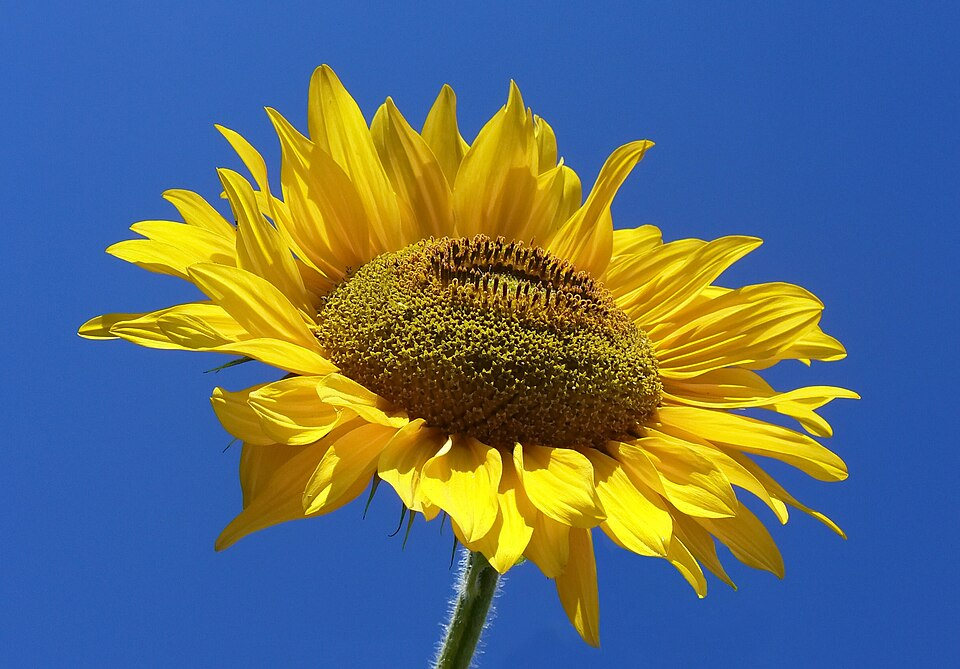
\includegraphics[width=0.5\textwidth]{img/test.jpg}
    \caption{Ảnh ví dụ (Nguồn: \url{wikipedia.org})}
    \label{fig:original_example}
\end{figure}

\subsection{Phép tích chập 2D (2D Convolution) và Xử lý biên (Padding)}

Nhiều thuật toán lọc ảnh đều dựa trên phép toán tích chập. Quá trình này sử dụng một ma trận nhỏ gọi là kernel kích thước $k \times k$ trượt dọc theo từng điểm ảnh của ảnh gốc. 

Đặc trưng cốt lõi của phép tích chập (để phân biệt với phép tương quan chéo - Cross-correlation) là kernel phải được lật ngược cả hai chiều ngang và dọc trước khi nhân với các điểm ảnh lân cận. Trong mã nguồn của đồ án, thao tác lật này được thực hiện trực tiếp thông qua việc truy xuất chỉ số ngược của mảng kernel.

\textbf{Xử lý vùng biên (Padding):}
Khi tâm của kernel nằm ở các điểm ảnh thuộc mép biên của ảnh gốc, một phần của kernel sẽ bị trượt ra bên ngoài ảnh (không có giá trị để tính toán). Để giải quyết vấn đề này, chương trình áp dụng kỹ thuật \textbf{Zero Padding}: mở rộng kích thước ảnh gốc bằng cách bao quanh ảnh bởi các viền pixel có giá trị bằng $0$. Số lớp viền cần thêm vào được tính bằng $pad = \lfloor k / 2 \rfloor$.

\textbf{Công thức:}
Giả sử ta có ảnh đầu vào $I$ đã được đệm bước Zero Padding và một kernel $K$ có kích thước $k \times k$ ($k$ là số lẻ). Giá trị của điểm ảnh mới $S(x, y)$ tại tọa độ $(x, y)$ sau khi thực hiện tích chập được tính theo công thức:

$$S(x, y) = \sum_{i=-pad}^{pad} \sum_{j=-pad}^{pad} I(x+i, y+j) \cdot K(-i, -j)$$

\textbf{Trong đó:}
\begin{itemize}
    \item $S(x, y)$: Giá trị cường độ sáng của điểm ảnh mới trên kết quả.
    \item $I(x+i, y+j)$: Giá trị cường độ sáng của điểm ảnh trên ảnh gốc tại vùng lân cận xung quanh tọa độ $(x, y)$.
    \item $K(-i, -j)$: Trọng số của kernel tại vị trí tương ứng đã được lật ngược theo cả hai chiều. Tâm của kernel được quy ước là tọa độ $(i = 0, j = 0)$.
\end{itemize}

\subsection{Chuyển đổi ảnh màu sang ảnh xám}

Để chuyển đổi ảnh màu RGB (đỏ, xanh lục, xanh lam) sang ảnh mức xám (Grayscale) ta dùng công thức tính giá trị mức xám $Y$ từ các kênh $R, G, B$ được định nghĩa như sau:

$$Y = 0.3 \times R + 0.59 \times G + 0.11 \times B$$

\textbf{Trong đó:}
\begin{itemize}
    \item $Y$: Cường độ sáng của điểm ảnh trên ảnh xám kết quả ($0 \le Y \le 255$).
    \item $R, G, B$: Giá trị cường độ của các kênh màu Đỏ, Xanh lá, Xanh lam của điểm ảnh gốc.
    \item Các hệ số $0.3, 0.59, 0.11$ (tổng bằng $1$) chính là các trọng số tương ứng với độ nhạy cảm của mắt người đối với từng dải phổ màu.
\end{itemize}

Ta sử dụng lệnh:

\begin{lstlisting}[language=bash, frame=single]
./bin/23122027 -rgb2gray <input_img_path> <output_img_path>
\end{lstlisting}

\textbf{Ví dụ minh họa:} Sau khi chuyển ảnh màu sang ảnh mức xám ta được

\begin{figure}[h!]
    \centering
    \begin{minipage}{0.48\textwidth}
        \centering
        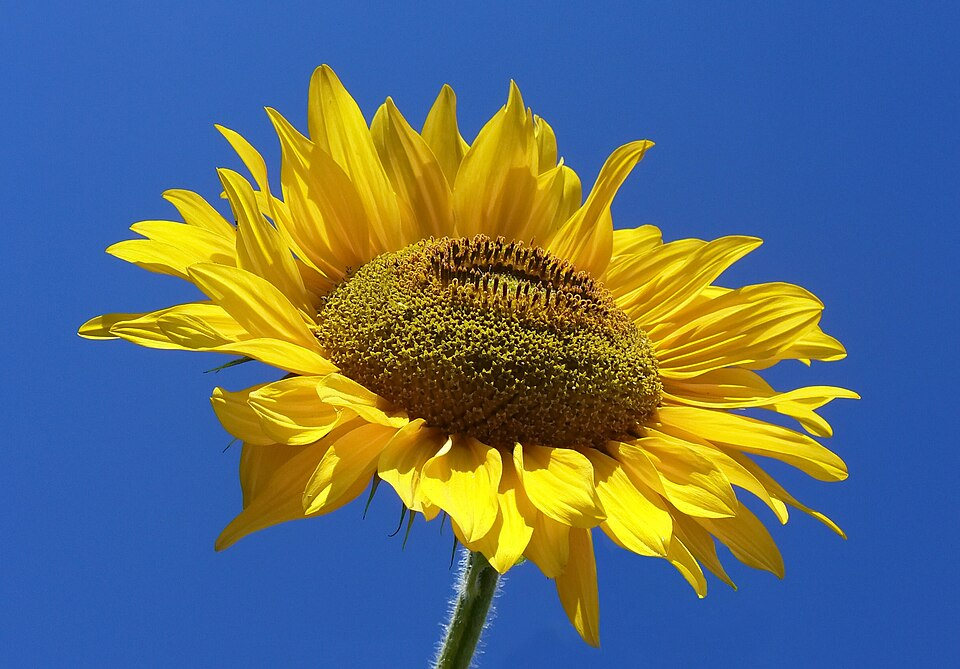
\includegraphics[width=\linewidth]{img/test.jpg}
        \centerline{(a) Ảnh gốc}
    \end{minipage}\hfill
    \begin{minipage}{0.48\textwidth}
        \centering
        
\includegraphics[width=\linewidth]{img/1_gray.jpg}
        \centerline{(b) Ảnh kết quả}
    \end{minipage}
    \caption{Kết quả chuyển đổi ảnh màu sang ảnh xám}
    \label{fig:gray_result}
\end{figure}

\subsection{Thay đổi độ sáng (Brightness)}

Để thay đổi độ sáng của ảnh, ta cộng thêm một hằng số $c$ vào giá trị cường độ của mỗi điểm ảnh. Kết quả sau đó được giới hạn trong khoảng $[0, 255]$ để tránh tràn giá trị.

$$I_{new}(x,y) = I_{old}(x,y) + c$$

\textbf{Trong đó:}
\begin{itemize}
    \item $I_{new}(x,y)$: Giá trị cường độ điểm ảnh mới.
    \item $I_{old}(x,y)$: Giá trị cường độ điểm ảnh ban đầu.
    \item $c$: Giá trị thay đổi độ sáng (nếu $c > 0$ ảnh sáng hơn, nếu $c < 0$ ảnh tối đi).
\end{itemize}

Ta sử dụng lệnh:
\begin{lstlisting}[language=bash, frame=single]
./bin/23122027 -brightness <input_img_path> <output_img_path> <c>
\end{lstlisting}

\textbf{Ví dụ minh họa:} Sau khi tăng độ sáng (c=50), ta được:
\begin{figure}[h!]
    \centering
    \begin{minipage}{0.48\textwidth}
        \centering
        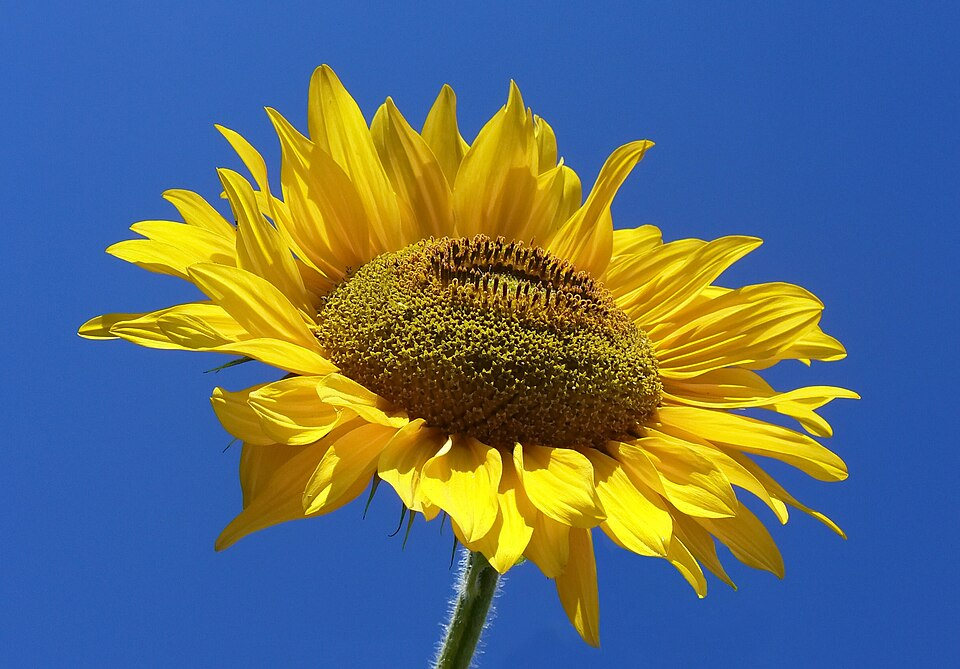
\includegraphics[width=\linewidth]{img/test.jpg}
        \centerline{(a) Ảnh gốc}
    \end{minipage}\hfill
    \begin{minipage}{0.48\textwidth}
        \centering
        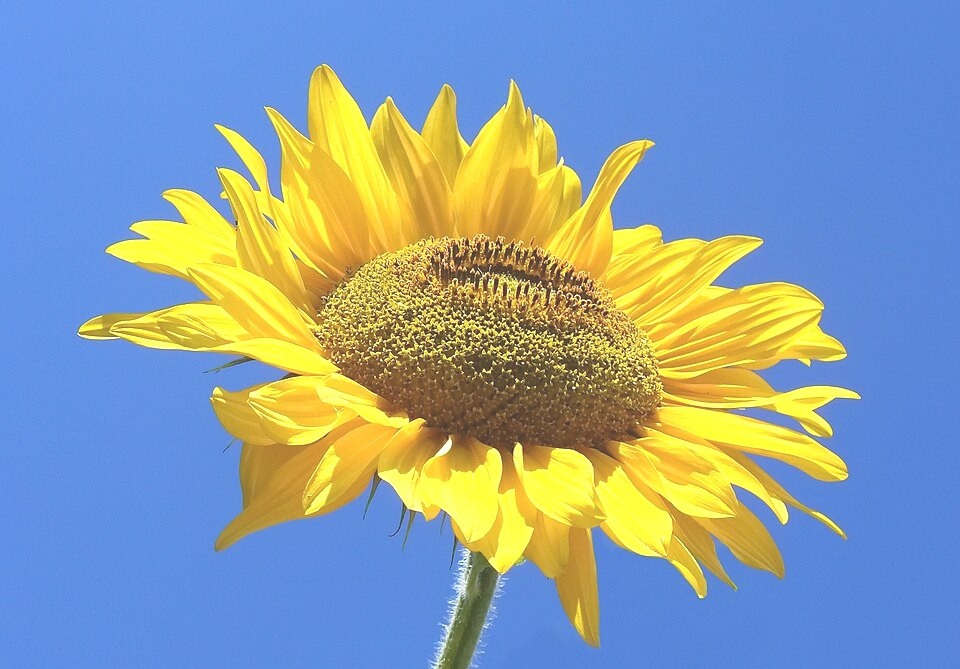
\includegraphics[width=\linewidth]{img/2_brightness_50.jpg}
        \centerline{(b) Ảnh kết quả}
    \end{minipage}
    \caption{Ảnh sau khi tăng độ sáng lên 50}
\end{figure}


\subsection{Thay đổi độ tương phản (Contrast)}

Để thay đổi độ tương phản, ta nhân giá trị cường độ của mỗi điểm ảnh với một hệ số $c$. Tương tự như độ sáng, kết quả được giới hạn trong khoảng $[0, 255]$.

$$I_{new}(x,y) = I_{old}(x,y) \times c$$

\textbf{Trong đó:}
\begin{itemize}
    \item $I_{new}(x,y)$: Giá trị cường độ điểm ảnh mới.
    \item $I_{old}(x,y)$: Giá trị cường độ điểm ảnh ban đầu.
    \item $c$: Hệ số tương phản ($c > 1$: tăng tương phản, $0 < c < 1$: giảm tương phản).
\end{itemize}

Ta sử dụng lệnh:
\begin{lstlisting}[language=bash, frame=single]
./bin/23122027 -contrast <input_img_path> <output_img_path> <c>
\end{lstlisting}

\textbf{Ví dụ minh họa:} Sau khi tăng độ tương phản (c=1.5), ta được:
\begin{figure}[h!]
    \centering
    \begin{minipage}{0.48\textwidth}
        \centering
        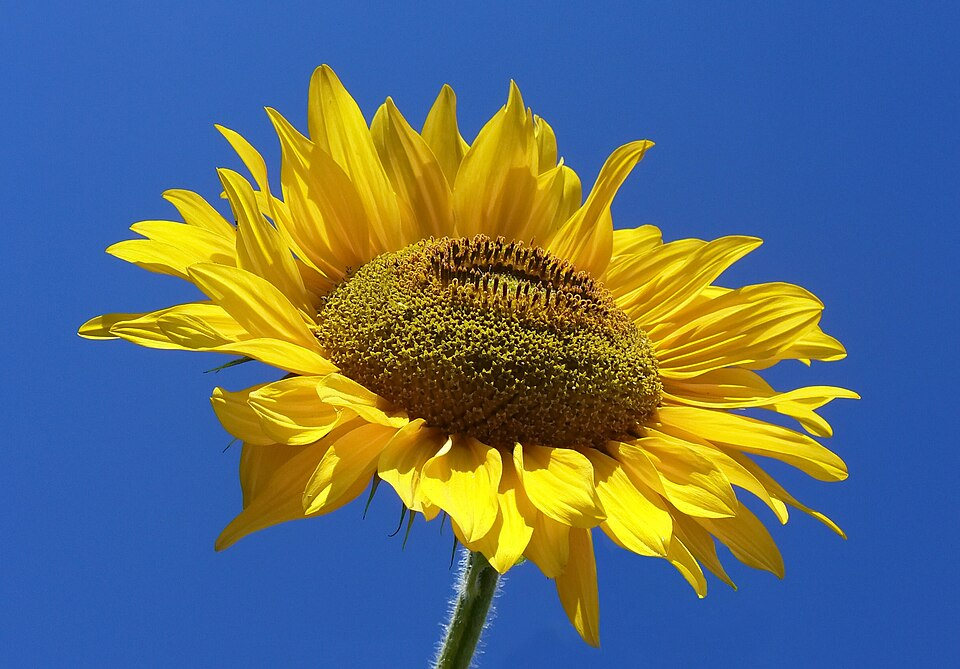
\includegraphics[width=\linewidth]{img/test.jpg}
        \centerline{(a) Ảnh gốc}
    \end{minipage}\hfill
    \begin{minipage}{0.48\textwidth}
        \centering
        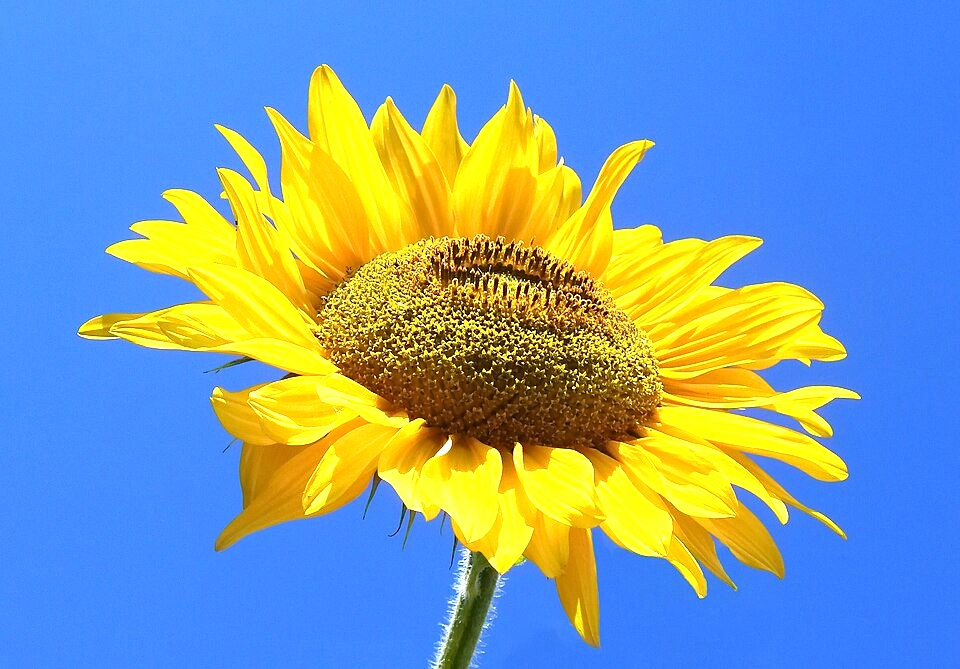
\includegraphics[width=\linewidth]{img/3_contrast_1.5.jpg}
        \centerline{(b) Ảnh kết quả}
    \end{minipage}
    \caption{Ảnh sau khi tăng độ tương phản 1.5 lần}
\end{figure}


\subsection{Bộ lọc trung bình (Average Filter)}

Bộ lọc trung bình là một bộ lọc không gian tuyến tính có tác dụng làm trơn ảnh và giảm nhiễu. Phương pháp này hoạt động bằng cách thay thế giá trị cường độ của mỗi điểm ảnh bằng trung bình cộng của các điểm ảnh trong một vùng lân cận kích thước $k \times k$.

Ta dùng một kernel $K$ kích thước $k \times k$, trong đó tất cả các phần tử đều có trọng số bằng nhau và bằng $\frac{1}{k^2}$:

$$K = \frac{1}{k^2} \begin{bmatrix} 1 & 1 & \cdots & 1 \\ 1 & 1 & \cdots & 1 \\ \vdots & \vdots & \ddots & \vdots \\ 1 & 1 & \cdots & 1 \end{bmatrix}_{k \times k}$$

\textbf{Trong đó:}
\begin{itemize}
    \item $k$: Kích thước của kernel lọc ($k$ là số lẻ nguyên dương, $k > 1$).
    \item Tổng các phần tử trong kernel $K$ luôn bằng $1$ để đảm bảo độ sáng trung bình của bức ảnh không bị thay đổi sau khi lọc.
\end{itemize}

Ảnh kết quả thu được bằng cách áp dụng phép tích chập 2D giữa ảnh gốc $I$ và kernel $K$ như đã định nghĩa ở phần trước.

Ta sử dụng lệnh:
\begin{lstlisting}[language=bash, frame=single]
./bin/23122027 -avg <input_img_path> <output_img_path> <k>
\end{lstlisting}

\textbf{Ví dụ minh họa:} Sau khi áp dụng bộ lọc trung bình ($k=5$), ta được:
\begin{figure}[h!]
    \centering
    \begin{minipage}{0.48\textwidth}
        \centering
        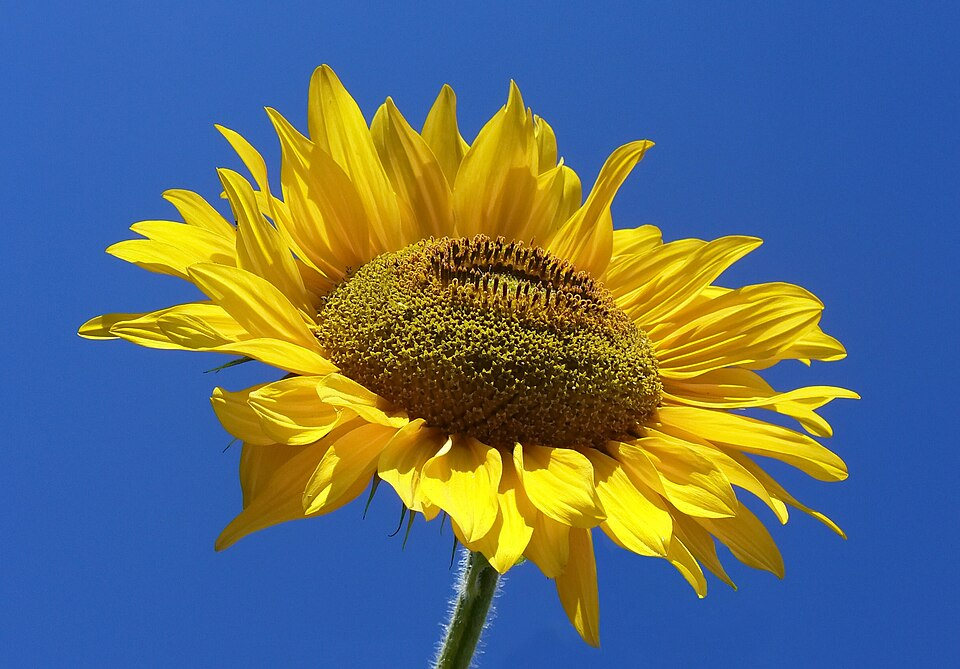
\includegraphics[width=\linewidth]{img/test.jpg}
        \centerline{(a) Ảnh gốc}
    \end{minipage}\hfill
    \begin{minipage}{0.48\textwidth}
        \centering
        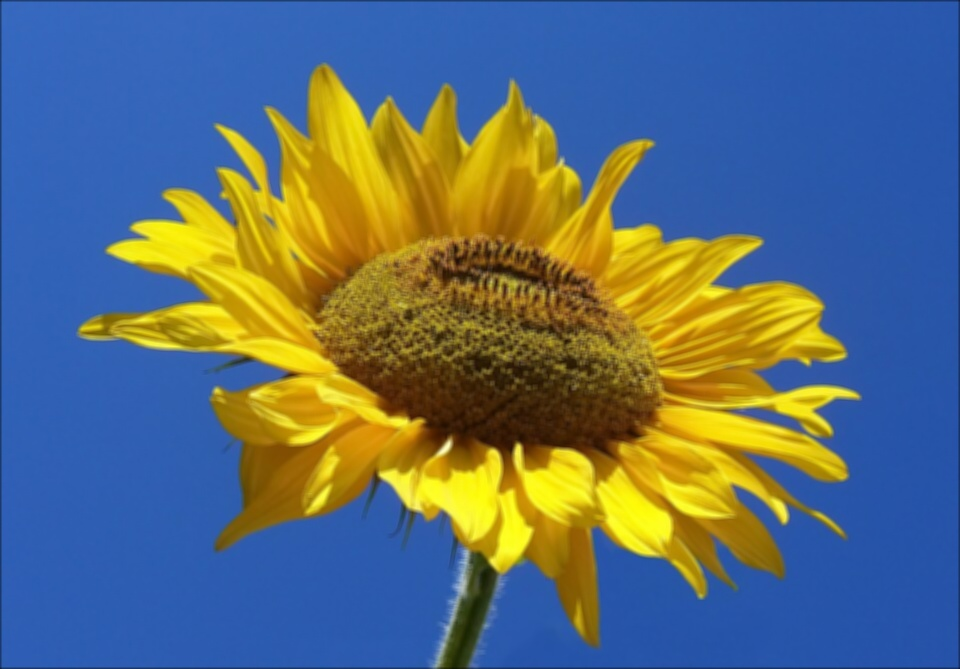
\includegraphics[width=\linewidth]{img/4_avg_k5.jpg}
        \centerline{(b) Ảnh kết quả}
    \end{minipage}
    \caption{Ảnh sau khi qua bộ lọc trung bình (k=5)}
\end{figure}


\subsection{Bộ lọc trung vị (Median Filter)}

Bộ lọc trung vị là một bộ lọc phi tuyến, cực kỳ hiệu quả trong việc loại bỏ nhiễu hạt (như nhiễu muối tiêu - salt and pepper) mà vẫn giữ được độ sắc nét của biên ảnh. Giá trị điểm ảnh được thay thế bằng giá trị trung vị của các điểm ảnh trong vùng lân cận $k \times k$.

$$I_{new}(x,y) = \text{median}\{I_{old}(x+i, y+j) \mid i, j \in [-pad, pad]\}$$

\textbf{Trong đó:}
\begin{itemize}
    \item $pad$: Bán kính lân cận, với $pad = \lfloor k/2 \rfloor$.
    \item $k$: Kích thước cửa sổ lọc ($k$ là số lẻ dương $> 1$).
\end{itemize}

Ta sử dụng lệnh:
\begin{lstlisting}[language=bash, frame=single]
./bin/23122027 -med <input_img_path> <output_img_path> <k>
\end{lstlisting}

\textbf{Ví dụ minh họa:} Sau khi áp dụng bộ lọc trung vị ($k=5$), ta được:
\begin{figure}[h!]
    \centering
    \begin{minipage}{0.48\textwidth}
        \centering
        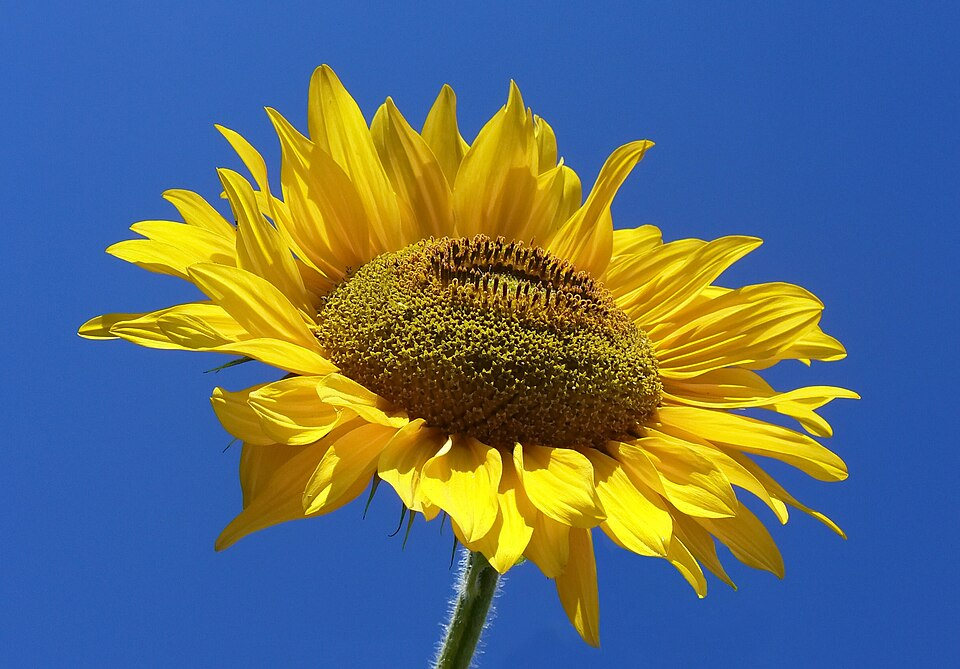
\includegraphics[width=\linewidth]{img/test.jpg}
        \centerline{(a) Ảnh gốc}
    \end{minipage}\hfill
    \begin{minipage}{0.48\textwidth}
        \centering
        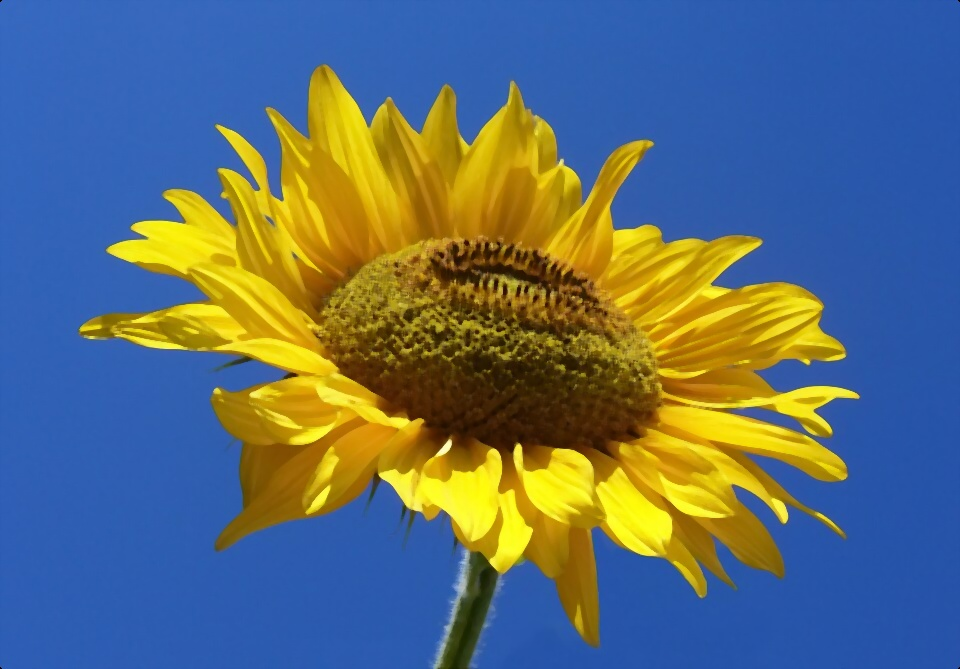
\includegraphics[width=\linewidth]{img/5_med_k5.jpg}
        \centerline{(b) Ảnh kết quả}
    \end{minipage}
    \caption{Ảnh sau khi qua bộ lọc trung vị (k=5)}
\end{figure}


\subsection{Bộ lọc Gauss (Gaussian Filter)}

Bộ lọc Gauss làm mờ ảnh bằng cách sử dụng một kernel tích chập mà trọng số của các phần tử giảm dần từ tâm ra biên theo phân bố chuẩn 2D. 

Trong đồ án này, để tự động hóa, độ lệch chuẩn $\sigma$ được tính toán trực tiếp dựa trên kích thước kernel $k$ (với $k$ lẻ) theo công thức:
$$\sigma = 0.3 \times \left(\frac{k - 1}{2} - 1\right) + 0.8$$

Trọng số ban đầu tại vị trí $(i, j)$ so với tâm của kernel (với $i, j \in [-pad, pad]$ và $pad = \lfloor k/2 \rfloor$) được tính bằng hàm phân bố Gauss:
$$G(i, j) = \frac{1}{2\pi\sigma^2} e^{-\frac{i^2 + j^2}{2\sigma^2}}$$

\textbf{Chuẩn hóa kernel (Normalization):} Để đảm bảo tổng các trọng số trong kernel bằng $1$ (tránh làm thay đổi độ sáng tổng thể của ảnh), mỗi phần tử trong kernel sẽ được chia cho tổng của tất cả các phần tử trước khi thực hiện phép tích chập:
$$K(i, j) = \frac{G(i, j)}{\sum_{u=-pad}^{pad} \sum_{v=-pad}^{pad} G(u, v)}$$

Ta sử dụng lệnh:
\begin{lstlisting}[language=bash, frame=single]
./bin/23122027 -gau <input_img_path> <output_img_path> <k>
\end{lstlisting}

\textbf{Ví dụ minh họa:} Sau khi áp dụng bộ lọc Gauss ($k=5$), ta được:
\begin{figure}[h!]
    \centering
    \begin{minipage}{0.48\textwidth}
        \centering
        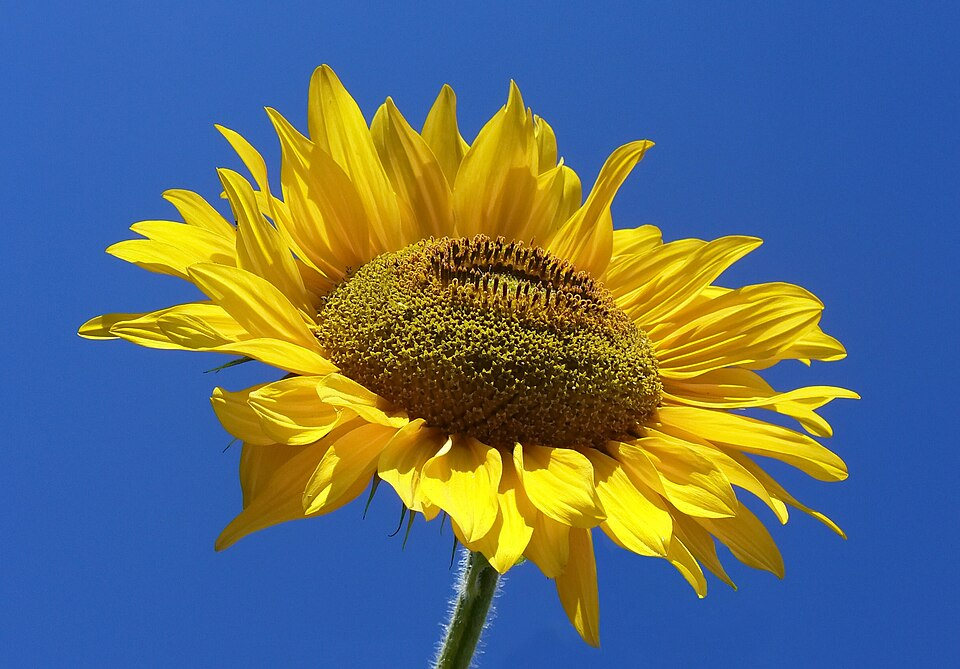
\includegraphics[width=\linewidth]{img/test.jpg}
        \centerline{(a) Ảnh gốc}
    \end{minipage}\hfill
    \begin{minipage}{0.48\textwidth}
        \centering
        
\includegraphics[width=\linewidth]{img/6_gau_k5.jpg}
        \centerline{(b) Ảnh kết quả}
    \end{minipage}
    \caption{Ảnh sau khi qua bộ lọc Gauss (k=5)}
\end{figure}


\subsection{Phát hiện biên cạnh bằng Sobel kernel (Sobel Edge)}

Toán tử Sobel phát hiện biên ảnh bằng cách tính xấp xỉ đạo hàm bậc nhất của cường độ sáng. Trước tiên, ảnh màu (nếu có) sẽ được chuyển sang ảnh mức xám. Sau đó, ảnh mức xám được tích chập lần lượt với hai kernel $3 \times 3$ để tìm gradient theo chiều ngang ($x$) và chiều dọc ($y$):

kernel gradient theo chiều ngang ($K_x$) và chiều dọc ($K_y$):
$$K_x = \begin{bmatrix} -1 & 0 & 1 \\ -2 & 0 & 2 \\ -1 & 0 & 1 \end{bmatrix}, \quad K_y = \begin{bmatrix} -1 & -2 & -1 \\ 0 & 0 & 0 \\ 1 & 2 & 1 \end{bmatrix}$$

Giả sử kết quả tích chập của ảnh gốc với $K_x$ và $K_y$ lần lượt là $G_x$ và $G_y$. Độ lớn gradient tại mỗi điểm ảnh được tính bằng căn bậc hai tổng bình phương của hai thành phần:
$$G = \sqrt{G_x^2 + G_y^2}$$
Kết quả cuối cùng $G$ sẽ được giới hạn về khoảng số nguyên $[0, 255]$ để hiển thị.

Ta sử dụng lệnh:
\begin{lstlisting}[language=bash, frame=single]
./bin/23122027 -sobel <input_img_path> <output_img_path>
\end{lstlisting}

\textbf{Ví dụ minh họa:} Sau khi phát hiện biên bằng Sobel, ta được:
\begin{figure}[h!]
    \centering
    \begin{minipage}{0.48\textwidth}
        \centering
        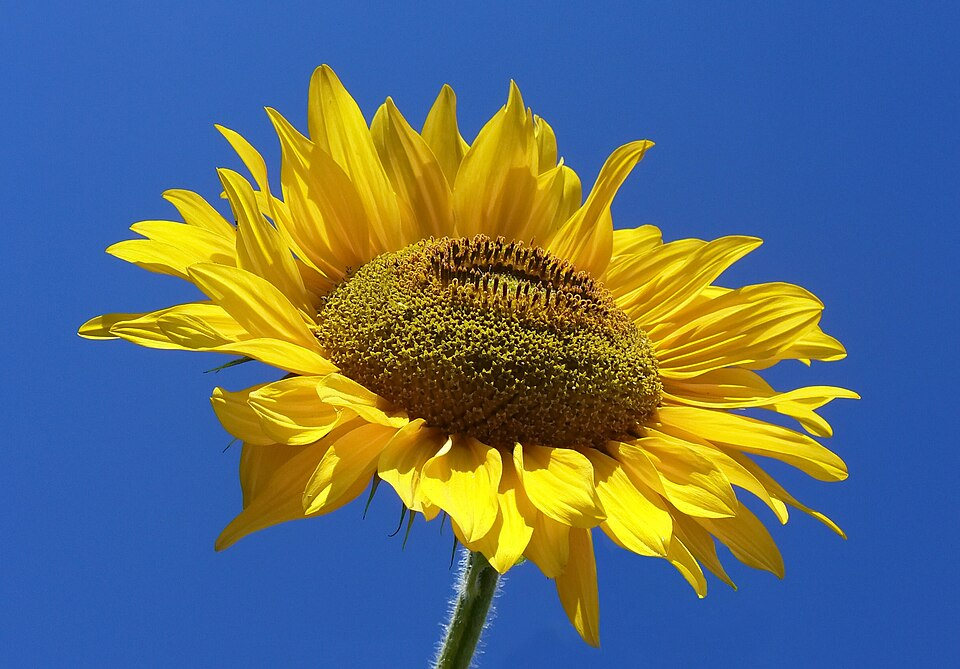
\includegraphics[width=\linewidth]{img/test.jpg}
        \centerline{(a) Ảnh gốc}
    \end{minipage}\hfill
    \begin{minipage}{0.48\textwidth}
        \centering
        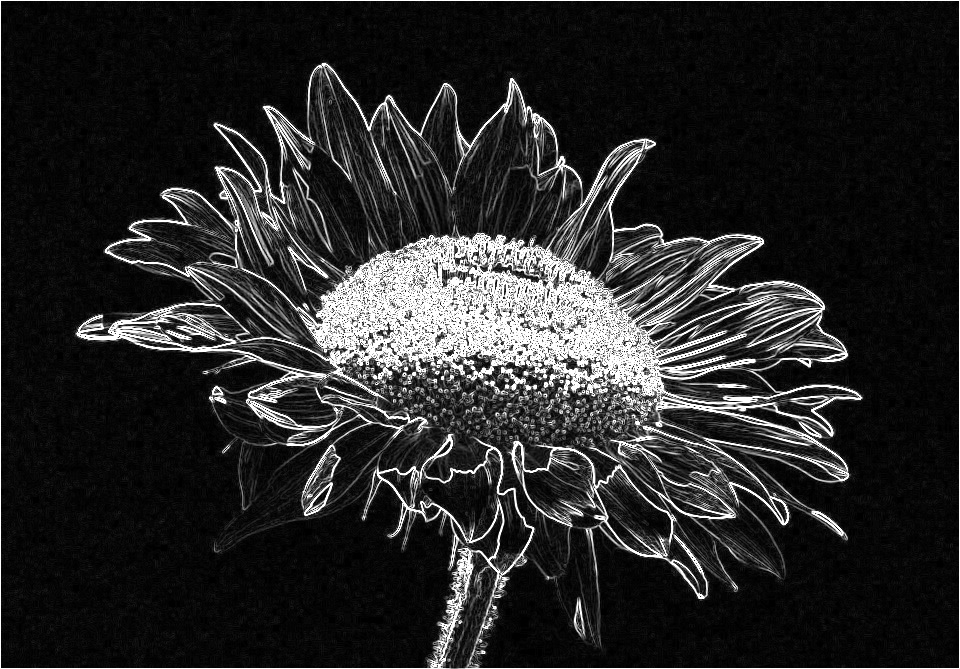
\includegraphics[width=\linewidth]{img/7_sobel.jpg}
        \centerline{(b) Ảnh kết quả}
    \end{minipage}
    \caption{Kết quả phát hiện biên Sobel}
\end{figure}


\subsection{Phát hiện biên cạnh bằng Laplace kernel (Laplace Edge)}

Toán tử Laplace sử dụng đạo hàm bậc hai để phát hiện biên, cho phép tìm biên trên mọi hướng (đẳng hướng) chỉ với một lần tích chập. Tương tự Sobel, ảnh đầu vào sẽ được chuyển sang mức xám trước khi xử lý.

Đồ án sử dụng ma trận kernel Laplace như sau:
$$K = \begin{bmatrix} 0 & 1 & 0 \\ 1 & -4 & 1 \\ 0 & 1 & 0 \end{bmatrix}$$

Đặc điểm của đạo hàm bậc hai là nó tạo ra các giá trị âm tại bề mặt chuyển từ sáng sang tối và giá trị dương tại bề mặt chuyển từ tối sang sáng. Do đó, sau khi áp dụng phép tích chập với ma trận $K$, chương trình thực hiện \textbf{lấy giá trị tuyệt đối} của toàn bộ các điểm ảnh để giữ lại thông tin biên ở cả hai chiều biến thiên, trước khi giới hạn về chuẩn 8-bit để hiển thị:
$$I_{new} = | I_{old} * K |$$

Ta sử dụng lệnh:
\begin{lstlisting}[language=bash, frame=single]
./bin/23122027 -laplace <input_img_path> <output_img_path>
\end{lstlisting}

\textbf{Ví dụ minh họa:} Sau khi phát hiện biên bằng Laplace, ta được:
\begin{figure}[h!]
    \centering
    \begin{minipage}{0.48\textwidth}
        \centering
        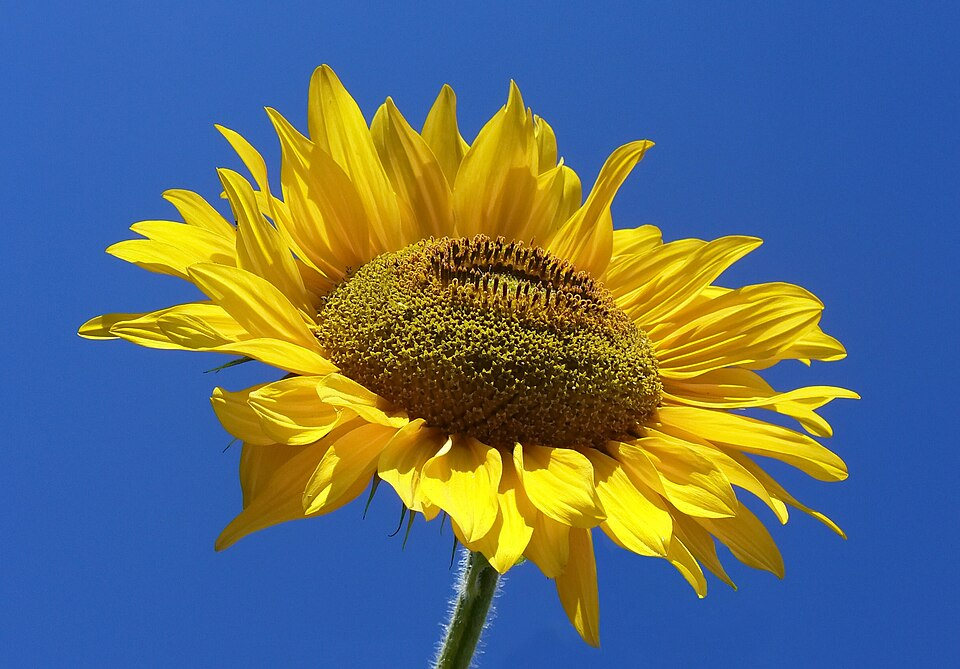
\includegraphics[width=\linewidth]{img/test.jpg}
        \centerline{(a) Ảnh gốc}
    \end{minipage}\hfill
    \begin{minipage}{0.48\textwidth}
        \centering
        
\includegraphics[width=\linewidth]{img/8_laplace.jpg}
        \centerline{(b) Ảnh kết quả}
    \end{minipage}
    \caption{Kết quả phát hiện biên Laplace}
\end{figure}

% References
\nocite{*}
\cleardoublepage
\phantomsection
\addcontentsline{toc}{section}{Tài liệu}
\bibliographystyle{plain}
\bibliography{content/ref}

% Appendix
% \appendix
% Add \cleardoublepage to move appendices to next page.
% \input{appendix/appendix.tex}
\end{document}